% KNAXS documentation for the Kassiopeia Guide
% B.Leiber email: benjamin.leiber@kit.edu
\section{Non-Axially-Symmetric Field Simulation: KNAXS}\label{sec:KNAXS}
  The \textbf{K}ATRIN \textbf{N}on-\textbf{Ax}ially-\textbf{S}ymmetric Field Simulation package consist of three main components:
  \begin{itemize}
    \item the calculation of the magnetic field of a thin, arbitrary current-carrying conductor via line-current-segments
    \item the calculation of the magnetic field of magnetic materials via magnetic dipoles
    \item a field-interpolation that uses the Hermite-3D interpolation method
  \end{itemize}
  % für weitere informationen auf DA verweisen ...
  %interpolation deswegen, weil die anderen methoden langsam sind ....
  
  \subsection{Line-segment discretization methods}
    \subsubsection{Integrated Biot-Savart}
    In the KATRIN experiment, there are a few components, generating magnetic fields that have a relatively simple shape, consisting of just a conductor that is shaped or wound in a distinct way. There are for example the components of the air coil system: the EMCS, that consists of several cosine coils and the LFCS that features some non-circular coils. Further applications will also include calculating the magnetic field of the dipole coils in the DPS1-R, DPS1-F and the rear section. To compute their effects on the magnetic field in the experiment the integrated Biot-Savart method is used. The magnetic field that is generated by any current-carrying component can be described using Biot-Savart’s law: From an infinitely long conductor segment with current $I$, an infinitesimally small segment $\mathrm d\vec{l}$ in direction of the current generates at the position $\vec{r}$ the magnetic field:
    \begin{equation}
      \mathrm d\vec{B} = \frac{\mu_0}{4\pi}\frac{I\mathrm d\vec{l}\times \hat{r}}{r^2}\text{.}
      \label{eq:biot savart}
    \end{equation}
    \begin{figure}[h]
      \centering \scalebox{1}{\includegraphics{images/KNAXSFigures/biot.pdf}}
      \caption{A line-current-segment is defined by a start point $A_1$, an endpoint $A_2$ and the magnitude of the current $\vec{I}$ that flows from $A_1$ to $A_2$.}
      \label{fig:definition line current segment}
    \end{figure}\\
    As we want to discretize our objects down to finite line-current segments, similar to the one shown in figure \ref{fig:definition line current segment}, we integrate along a line current segment and get:
    \begin{equation}
      \begin{aligned}
      \vec{B}_{i} &= \frac{\mu_0}{4\pi} \mathrm{d}\vec{L} \times \vec{I} \qquad \text{with} \\
      \mathrm{d}\vec{L} &= \left(\frac{\hat{r}_{1}+\hat{r}_{2}}{R+l}-\frac{\hat{r}_{1}+\hat{r}_{2}}{R-l}\right)\text{,} \\
      R&=|\vec{r}_{1}|+|\vec{r}_{2}| \text{,}\qquad l=|\vec{r}_{2}-\vec{r}_{1}|\qquad\text{and}\qquad \hat{r}_i = \frac{\vec{r}_i}{|\vec{r}_i|}\text{.}
      \end{aligned}
    \end{equation}
    Being able to use the superposition principle, it is possible to approximate complex shapes by numerous line-current-segments and simply sum up their individual field contributions $\vec{B}_{i}$ to get the overall resulting magnetic field:
    \begin{equation}
      \vec{B}_{total}=\sum_{i=1}^{N} \vec{B}_i
    \end{equation}
    Geometries composed of such line current segments can easily be tested by checking the validity of the Maxwell-equations. If, for example, the curl of the magnetic field $\vec{\nabla}\times\vec{B}_{total}$ is non-zero in vacuum, this is a hint that a current loop is not closed and that you should check your discretization.

    \subsubsection{Magnetic Dipole-Bars}
      The hall where the KATRIN experiment is housed consists mainly of concrete and ferro-magnetic steel. The steel rods inside the floor and the walls cause non-negligible, highly inhomogeneous magnetic stray-fields. As people have already foreseen that during the planning of the experiment, the KATRIN-hall was partially built with stainless steel that has a by far decreased magnetisation. However, there remains a strong magnetic component caused by the magnetic materials in the walls of the KATRIN-hall. \\
      Fortunately, it is known how the obstructed steel bars are magnetized: namely along their symmetry axis. In this case, one can make the simplifying approximation of a magnetic dipole with two magnetic charges $Q$ at both ends of the bar (see figure \ref{fig:definition magnetic dipole bar}).
      \begin{figure}[h]
	\centering \scalebox{0.9}{\includegraphics{images/KNAXSFigures/mag_bar.pdf}}
	\caption{The magnetic-dipole-bars are characterised by two magnetic charges at the ends of the bar, their distance and the radius of the bar.}
	\label{fig:definition magnetic dipole bar}
      \end{figure}\\
      The magnetic field of such a dipole can be easily calculated analogue to Coulomb's law:
      \begin{equation}
	\vec{B}_{i}(P) = -Q \frac{\mu_0}{4\pi}\left(\frac{\vec{r}_{a}}{|\vec{r}_{a}|^3}+\frac{\vec{r}_{b}}{|\vec{r}_{b}|^3}\right) \qquad \text{with} \qquad Q = |\vec{M}| \cdot\pi r^2
      \end{equation}
      $\vec{M}$ denotes the magnetisation and $r$ the radius of the dipole-bar. Again, to get the total magnetic field from all dipole-bars their contributions $B_{i}$ have to be summed up.
  \subsection{Three-Dimensional Hermite-Interpolation} % ZITAT M. EUPNER !!!!!!!!
    Interpolation methods are often employed when calculating the field of a static setup. The interpolation grid is plotted once in advance and every time the field needs to be evaluated in a certain point, it is interpolated and optionally scaled using the precomputed grid. The Hermite-interpolation, in contrast to the linear-interpolation does not only need the values at the grid points, but also their partial derivates. This results in a longer precomputation time, but as the accuracy of the Hermite-interpolation scales not just with the 2nd but with the 4th power of the grid distance, this is the preferred method to use when interpolating with relatively large grids. \\  
    Interpolating usually means a dramatic speed up of the field calculations, especially for non axisymmetric fields and still grants a high numeric precision.
  \subsubsection{Theory}
    \begin{figure}[h]
      \centering \scalebox{0.6}{\includegraphics{images/KNAXSFigures/cuboid.pdf}}
      \caption{Example grid consisting of cuboids.}
      \label{fig:grid of cuboids}
    \end{figure}
    We are given a rectangular, three-dimensional grid that consists of cuboids (see fig. \ref{fig:grid of cuboids}. A cuboid Q of this grid can be described as follows.
    \begin{equation}
	    Q := \left\lbrace \left( x_{1},x_{2},x_{3} \right) ~ \epsilon ~  \mathbb{R}^{3} \;  / \;  x_{ui} < x_{i} < x_{oi} \;  ; \;  i=1,2,3  \right\rbrace 
    \end{equation}
    Through a coordinate-transformation of the form:
    \begin{equation}
	    \begin{aligned}
		    u_{i} &= \frac{x_{i}-x_{mi}}{a_{i}} \quad  \text{with} \\
		    x_{mi} &= \frac{x_{oi}+x_{ui}}{2} \quad  \text{and} \quad  a_{i} = \frac{x_{oi}-x_{ui}}{2}
	    \end{aligned}
    \end{equation}
    we project $Q$ to the unit-cube $E$:
    \begin{equation}
	    E := \left\lbrace \left( u_{1},u_{2},u_{3} \right) ~ \epsilon ~  \mathbb{R}^{3} \;  / \;  -1 < u_{i} < 1 \;  ; \;  i=1,2,3  \right\rbrace
    \end{equation}
    Now we define a function $g(\vec{u})$ on $E$ with:
    \begin{equation}
	    f(\vec{x}) = g(\vec{u}(\vec{x}))
    \end{equation}
    The goal is to interpolate $g(\vec{u})$ within the unit-cube $E$. Therefore, we need to know the function-values at the eight corner points $\vec{u}_{i}$ as well as their first partial derivatives. We combine them into a Matrix $\mathcal{G}$, where the function-values fill one column:
    \begin{equation}
	    \mathcal{G}_{i0} := g(\vec{u}_{i}) ~ (i=1,...,8)
    \end{equation}
    and the others are filled by their partial derivatives:
    \begin{equation}
	    \mathcal{G}_{ij} := \left\lbrace \frac{\partial g(\vec{u})}{\partial u_{j}} \right\rbrace_{\vec{u}=\vec{u}_{i}} \quad (i=1,...,8 \; ; \; j=1,2,3)
    \end{equation}
    The next step is to define a so called Interpolation-polynomial:
    \begin{equation}
	    G(\vec{u})= \sum_{i=1}^{8} \sum_{j=0}^{3} \mathcal{G}_{ij} \phi_{ij}(\vec{u})
    \end{equation}
    The coefficient-polynomials $\phi_{ij}$ are chosen, so that $G(\vec{u}_{k})=\mathcal{G}_{k0}$ and \\$\left\lbrace \frac{\partial g(\vec{u})}{\partial u_{1}} \right\rbrace_{\vec{u}=\vec{u}_{k}} = \mathcal{G}_{k1}$. This leads to the following constraints:
    \begin{equation}
    \phi_{ij}(\vec{u}_{k})=\delta_{ik}\delta_{j0} \qquad \mbox{and} \qquad \left\lbrace \frac{\partial \phi_{ij}(\vec{u})}{\partial u_{1}} \right\rbrace_{\vec{u}=\vec{u}_{k}} =\delta_{ik}\delta_{j1}
    \end{equation}
    These are fulfilled, if we define $\phi_{ij}$ like:
    \begin{equation}
	    \phi_{ij}(\vec{u}) := u_{ij} \prod_{k=1}^{3} \varphi_{jk} (u_{ik} \cdot \vec{u}_{k})
    \end{equation}
    where $\varphi_{jk}$ is given by:
    \begin{equation}
	    \varphi_{jk}(t) := \frac{1}{4} \left[ \left( 2+3t-t^{3}\right) + \left( -3-4t+t^{2}+2t^{3}\right) \delta_{jk} \right] \quad \mbox{and} \quad u_{i0}:=1
    \end{equation}
    \\
    In order to interpolate the function $f(\vec{x})$ within the cuboid $Q$, we have to follow some simple steps:
    \begin{enumerate}
	    \item calculate the function-values and their partial derivatives of $f$ regarding $\vec{x}$ at all 8 corner points,
	    \item transform them into the unit-cube $E$:
		    \begin{equation}
		    \mathcal{G}_{ij} =
		    \begin{cases}
			    a_{j} \cdot \left\lbrace \frac{\partial f(\vec{x})}{\partial x_{j}} \right\rbrace_{\vec{x}=\vec{x}_{i}} & \text{if} \quad j>0 \\
			    f(\vec{x}_{i}) & \text{if} \quad j=0
		    \end{cases}
		    \end{equation}
	    \item and interpolate function-values and derivatives at any point $\vec{x} ~ \epsilon ~ Q$ :
		    \begin{equation}
		    \begin{aligned}
			    \frac{\partial f(\vec{x})}{\partial x_{j}} &= a_{j}^{-1} \cdot \frac{\partial G(\vec{u}(\vec{x}))}{\partial u_{j}} \qquad j=1,2,3 \\
			    f(\vec{x}) &= G(\vec{u}(\vec{x}))
		    \end{aligned}
		    \end{equation}
    \end{enumerate}
    Interpolation methods  yield the possibility of a scalable precision. When a high precision is needed, the distance between the grid points can be chosen very small and in the contrary case, when a lower precision is sufficient, it can be chosen rather large. This has no impact on the actual computation time, just on the time needed to compute the initial grid.
    \subsection{Implementation}
      All KNAXS-classes derive from the \texttt{Field} base-class and \texttt{Magfield} respectively. The integrated Biot-Savart method is implemented in a class called \texttt{BiotSavart} and the field calculation of the magnetic dipole-bars in a class called \texttt{MagMaterials}. They are both organized in a very similair way: They both have a member-container that holds their particular segments:
      \begin{itemize}
	\item \texttt{Line(Double\_t current, TVector3 startPosition, TVector3 endPosition)} represents a line-current segment that is defined through to points and a current running from one point to the other. It has methods to set and get the start- and endpoint of the line and the current it is carrying. \texttt{FieldInLine(TVector3 p)} returns the magnetic field ($\vec{B}$) caused by the segment at the position \texttt{p}.
	\item \texttt{Bar(TVector3 P1, TVector3 P2, Double\_t magnetization, Double\_t radius, Double\_t susceptibility)} represents a magnetized bar and is defined through two points at the end, a magnetization pointing from one point to the other, a radius and the magnetic susceptibility of the material. It has methods to get and set these quantities. \texttt{GetHField(TVector3 p)} returns the magnetic field ($\vec{H}$) caused by the segment at the position \texttt{p}.
      \end{itemize}
      These elements can be added to the field-objects through the \texttt{AddLine(Line)}/\texttt{AddBar(Bar)} methods. The total magnetic field at a given position can be retrieved through the \texttt{GetField(TVector3)} method. In this method, the contributions of the single elements are simply summed up and the total field is then returned.
      \\
      The interpolation classes are a bit more complicated. The base method was implemented into the class \texttt{FieldInterpolation}. The classes \texttt{MagfieldInterpolate} and \texttt{ElfieldInterpolate} inherit from this class, and of course from the abstract field base classes. Figure \ref{fig:Magfieldinterpolate overview} shows a principle diagram of the \texttt{MagfieldInterpolate} class and figure \ref{fig:Elfieldinterpolate overview} of the \texttt{ElfieldInterpolate} class, respectively.
      \begin{figure}[h]
		\centering 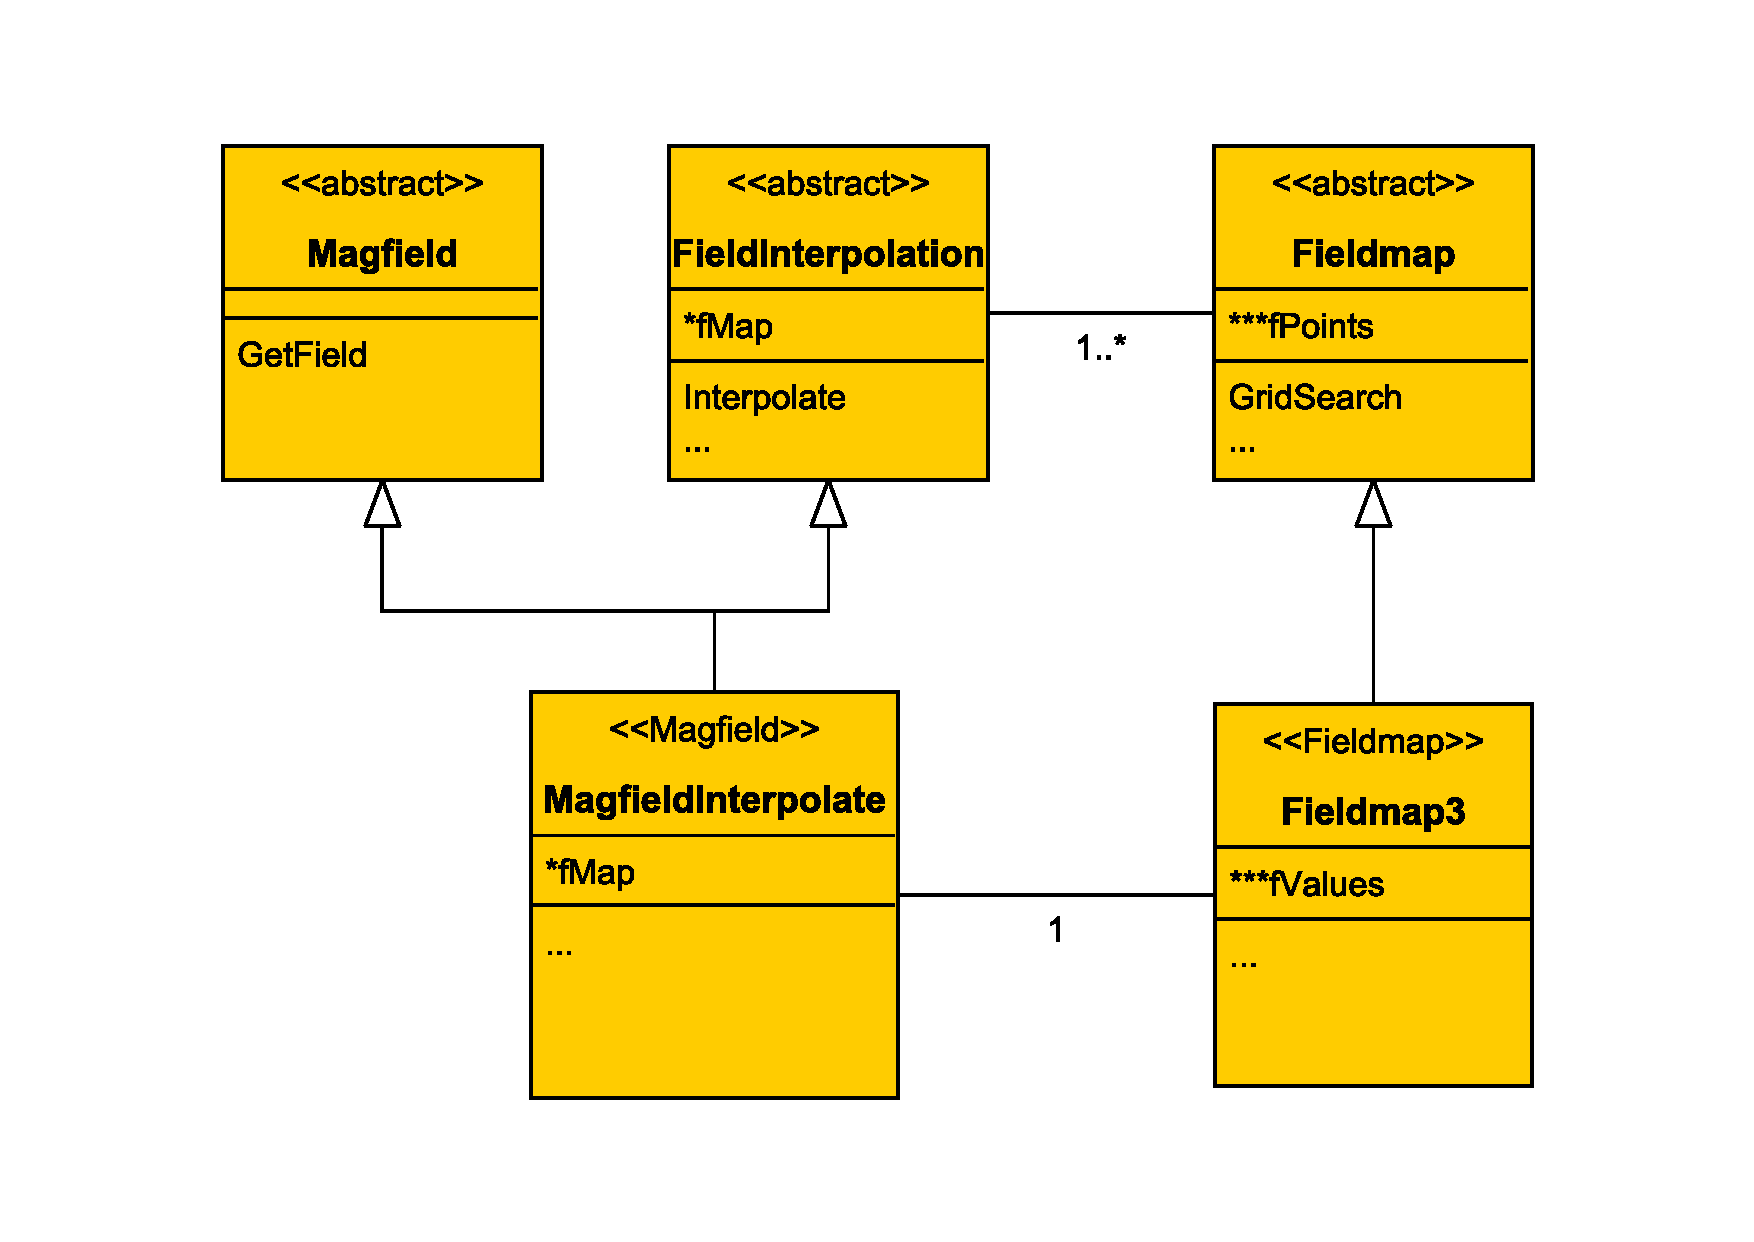
\includegraphics[width=0.9\textwidth]{images/KNAXSFigures/mag_interpolation_uml.pdf}
		\caption{Overview of the \texttt{MagfieldInterpolate} class: It inherits from the abstract classes \texttt{Magfield} and \texttt{FieldInterpolation}. It has one member object of the class \texttt{Fieldmap3} that inherits from the abstract class \texttt{Fieldmap}.}
		\label{fig:Magfieldinterpolate overview}
      \end{figure}
      Objects of the stereotype \texttt{FieldInterpolation} store one or more interpolation grids in objects of the stereotype \texttt{Fieldmap}. These grids contain for example the scalar electric potential with just one value at a grid point in case of a \texttt{Fieldmap1} object, and the grids for the three-dimensional vector fields, that have three values and nine partial derivatives in one grid point, are stored in  \texttt{Fieldmap3} objects. In case of rotational symmetry, one can also use the \texttt{Fieldmap2} objects, but this has to be specified explicitly by the user.
      \begin{figure}[h]
		\centering 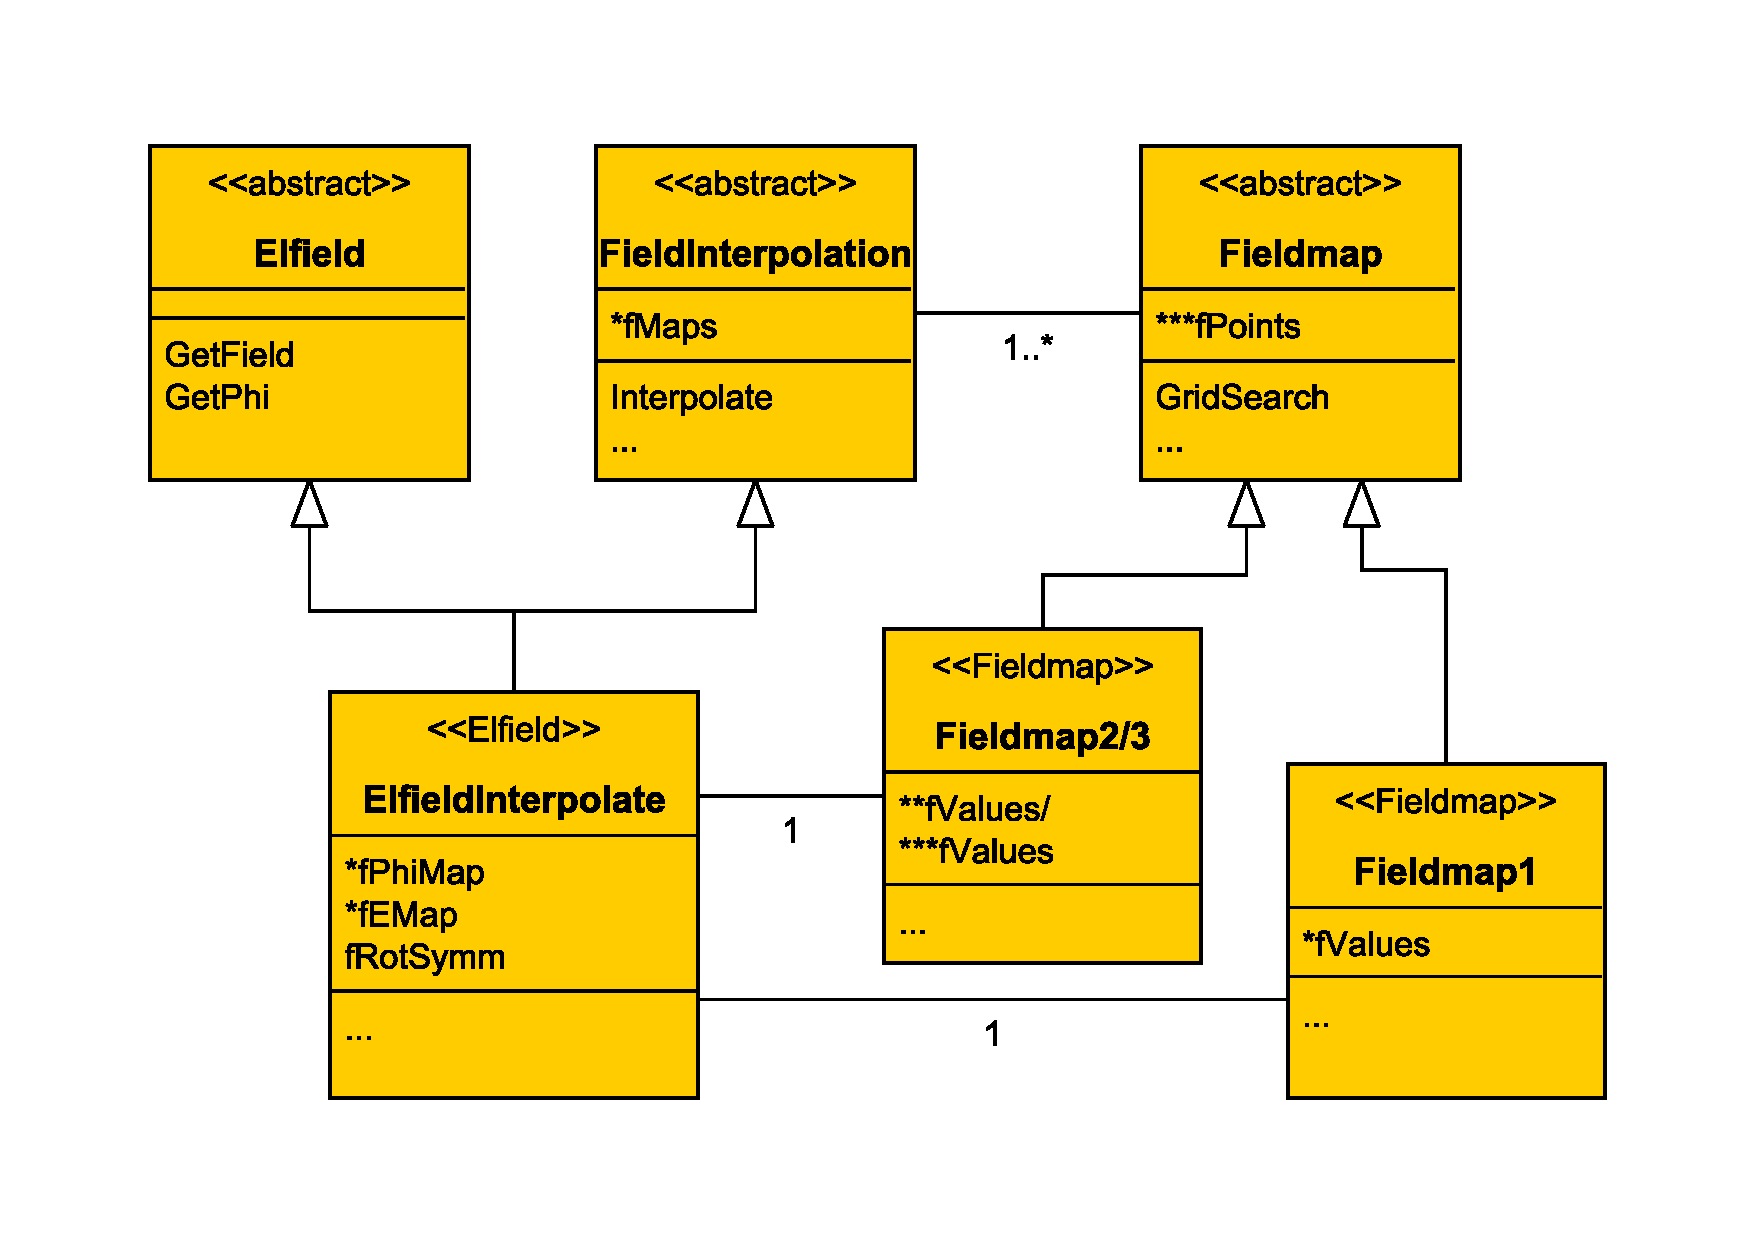
\includegraphics[width=0.9\textwidth]{images/KNAXSFigures/el_interpolation_uml.pdf}
		\caption{Overview of the \texttt{ElfieldInterpolate} class: It inherits from the abstract classes \texttt{Elfield} and \texttt{FieldInterpolation}. It has two member objects that inherit from the abstract class \texttt{Fieldmap}: a \texttt{Fieldmap1} object, in which the interpolation grid for the electric potential is stored and a \texttt{Fieldmap2} or \texttt{Fieldmap3} object, depending if the field is axially symmetric, in which the interpolation grid for the electric field is stored.}
		\label{fig:Elfieldinterpolate overview}
      \end{figure}
      In order to pre-compute a grid, the virtual methods \texttt{CreateMagFieldmap} and \texttt{CreateElFieldmap} that are members of the \texttt{Fieldmap} classes have to be called. They compute a grid of the specified \texttt{Magfield} or \texttt{Elfield} object, respectively. \texttt{CreateElfieldmap} actually creates two field maps, one for the electric field and one for the potential. Afterwards they are saved to a file and can be read in with the virtual method \texttt{ReadMapFromFile}.